\section{Diskussion}
\label{sec:Diskussion}

In der Auswertung kam es bereits zu einigen Unrelistischen und offensichtlichen
falschen Werten die aus alle aus Berechnungen stammten.
Im Folgenden soll die Ursache für die dramastischen Abweichungen analysiert werden.


Dafür soll zu Beginn die Messung an sich überprüft werden.
Dazu betrachte man sich, die jeweilige theoretische Schwingungsdauer und 
vergleich diese mit den gemessenen Schwnungsdauern.
\begin{figure}
    \centering
    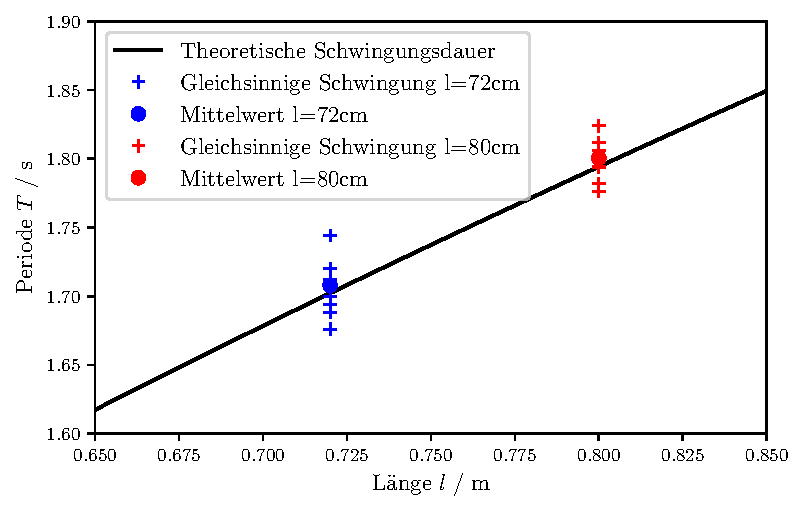
\includegraphics[width=0.5\textwidth]{plot1.pdf}
    \caption{Gleichsinnige Schwingungen}
\end{figure}

\begin{figure}
    \begin{subfigure}[c]{0.5\textwidth}
        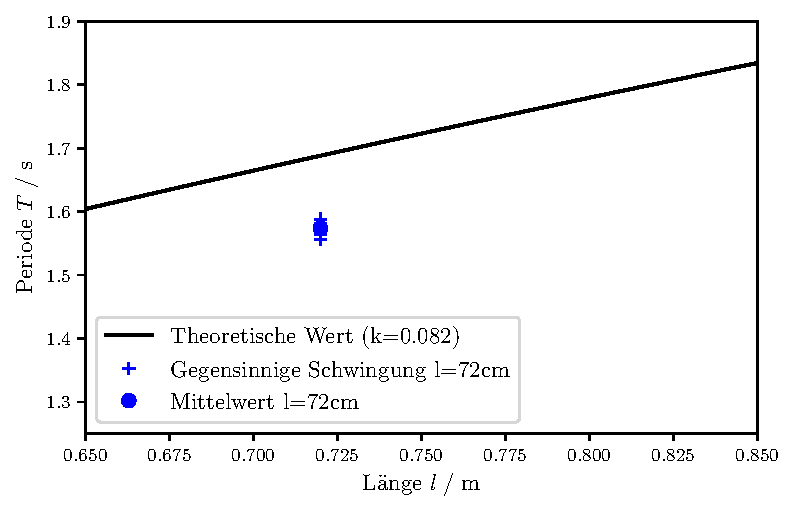
\includegraphics[width=\textwidth]{plot2.pdf}
        \subcaption{Pedel 72cm}
    \end{subfigure}
    \begin{subfigure}[c]{0.5\textwidth}
        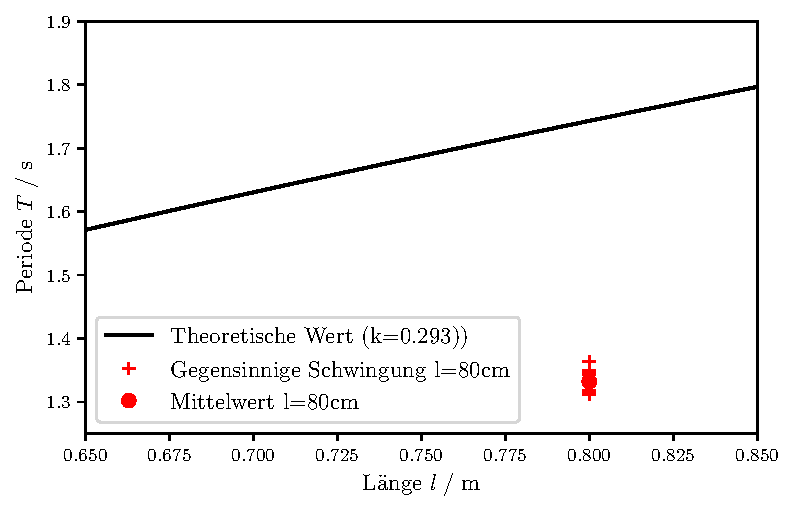
\includegraphics[width=\textwidth]{plot3.pdf}
        \subcaption{Pendel 80cm}
        \label{subfig:pedel80}
    \end{subfigure}
    \caption{Gleichsinnige Schwingungsdauer}
\end{figure}

Dabei ergibt sich der zu erwartende Theoretische Werte aus Geichung (8!).

Hier bei wird besonders gut deutlich, dass bei \ref{subfig:pendel80}, große Abweichungen
vorliegen. Dies lässt sich nur auf einen Messfehler zurückführen.
Weiterführend sei zu beachten, dass die Kopplungskonstante die für die theoretische Kurve
verwendet wird, ebenfalls aus diesen falschen Werten stammt.

Dies erklärt weiterführend, warum die Kopplungskonstant aus \ref{eqn:kopplung80} nicht die selben
sind, bzw. warum die Konstante resultierend aus den Schwingsungsdauern der Pedellänge 80cm so weit von der
Kopplungskonstanten die aus Schwingunsdauern des Pendel mit einer Länge von 72cm enfernt ist.

Fazit: Der Messfehler der Gegensinnigen Schwingung von der Pendellänge $l=80cm$ ist 
ist ein Ursprung der 